\thispagestyle{hoccungpinone}
\pagestyle{hoccungpi}
\everymath{\color{hoccungpi}}
\graphicspath{{../hoccungpi/pic/}}
\blfootnote{$^*${\color{hoccungpi}Dựa trên bài giảng của tác giả tại trường THPT chuyên Quốc học Huế, tháng $5/2022$.}}
\blfootnote{$^1${\color{hoccungpi}Viện Toán học.}}
\begingroup
\AddToShipoutPicture*{\put(0,616){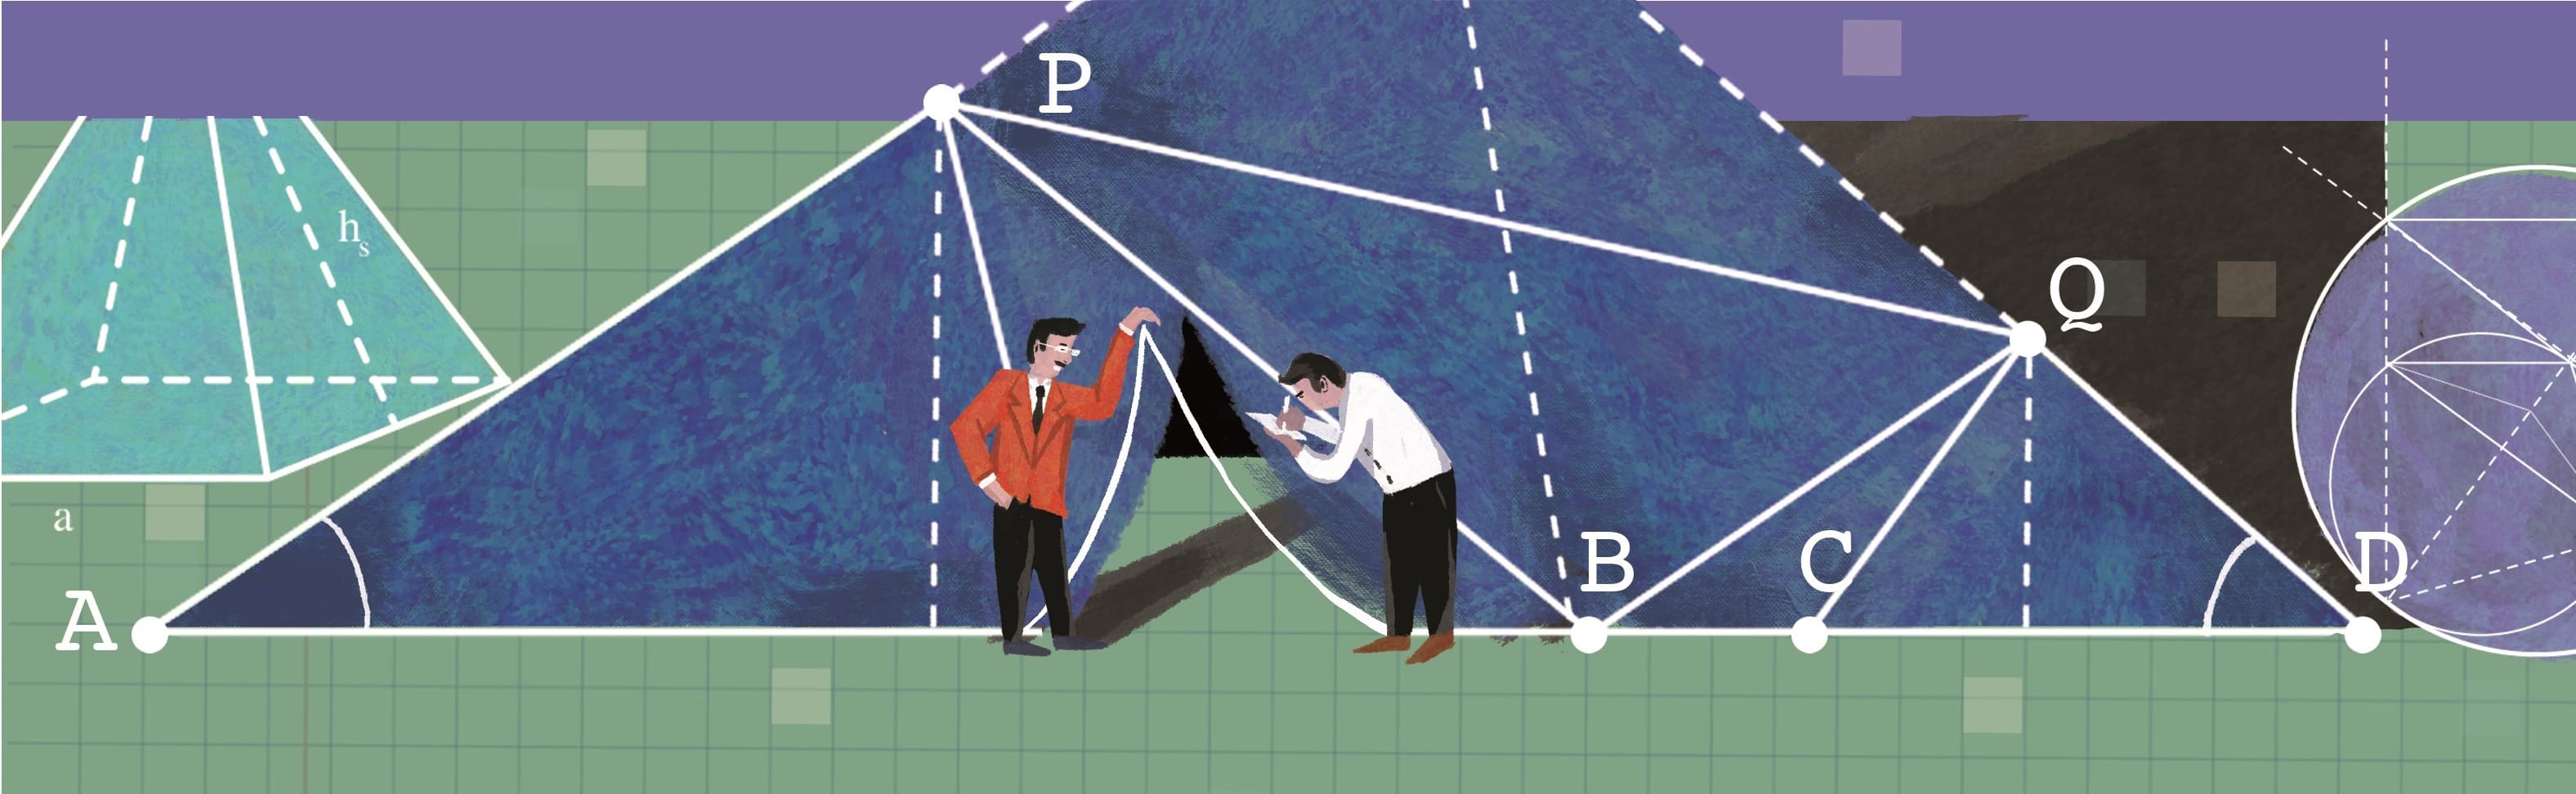
\includegraphics[width=19.3cm]{../bannerhoccungpi}}} 
\AddToShipoutPicture*{\put(115,520){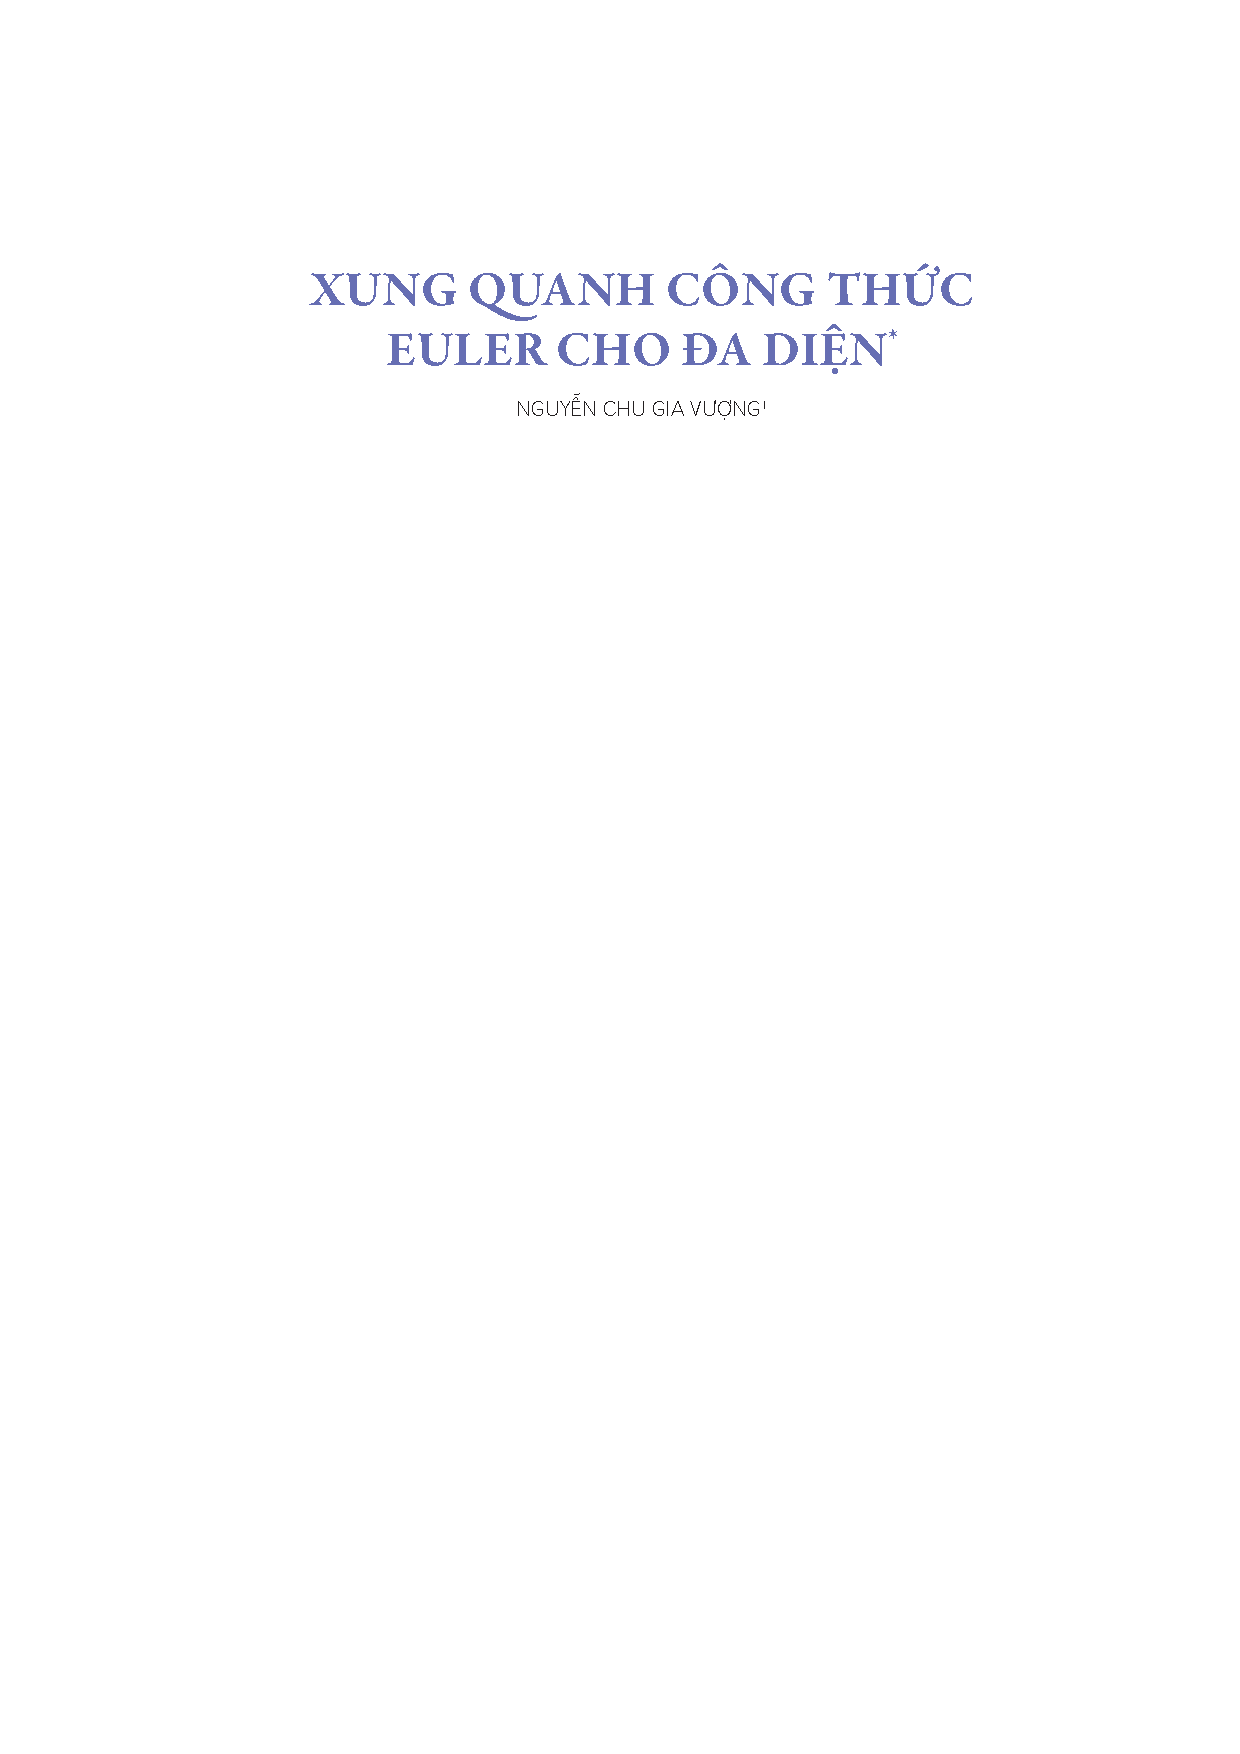
\includegraphics[scale=1]{../tieude.pdf}}} 
\centering
\endgroup
\vspace*{185pt}

\begin{multicols}{2}
%	\setlength{\abovedisplayskip}{5pt}
%	\setlength{\belowdisplayskip}{5pt}
	\textbf{\color{hoccungpi}Công thức Euler cho đa diện}
	\vskip 0.1cm
	Các khối đa diện là đối tượng hình học rất quen thuộc với mỗi người. Nhắc lại rằng, một đa diện lồi trong không gian ba chiều là một hình khối trong không gian mà các mặt là các đa giác lồi. Kết quả mà chúng ta quan tâm trong bài viết này là được phát biểu sau đây.
	\vskip 0.1cm
	\textbf{\color{hoccungpi}Định lý} $\pmb{1}$ (Công thức Euler)\textbf{\color{hoccungpi}.} \textit{Gọi $v$, $e$ và $f$ tương ứng là số đỉnh, số cạnh và số mặt của  một khối đa diện lồi $P$. Khi đó}
	\begin{align*}
		v-e+f=2.
	\end{align*}
	\begin{figure}[H]
		\centering
		\vspace*{-5pt}
		\captionsetup{labelformat= empty, justification=centering}
		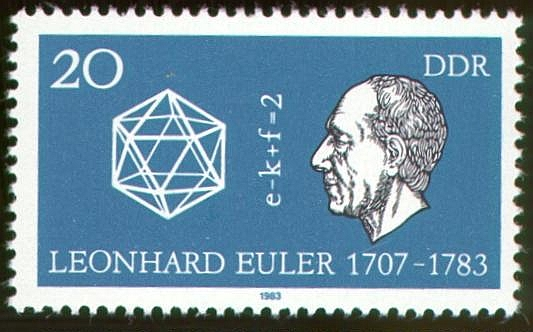
\includegraphics[width=1\linewidth]{Euler_GDR_stamp}
		\caption{\small\textit{\color{hoccungpi}Leonhard Euler ($1707-1783$) là một nhà toán học, nhà vật lý, nhà thiên văn học, nhà địa lý, nhà logic và kỹ sư người Thụy Sĩ.}}
		\vspace*{-10pt}
	\end{figure}
	Trước khi trình bày chứng minh, ta hãy kiểm tra công thức Euler cho một số đa diện quen thuộc.
	\vskip 0.1cm
	\textbf{\color{hoccungpi}Ví dụ} $\pmb{1.}$
	\vskip 0.1cm
	\textit{$1.$ Tứ diện
	\begin{figure}[H]
		\centering
		\vspace*{-5pt}
		\captionsetup{labelformat= empty, justification=centering}
		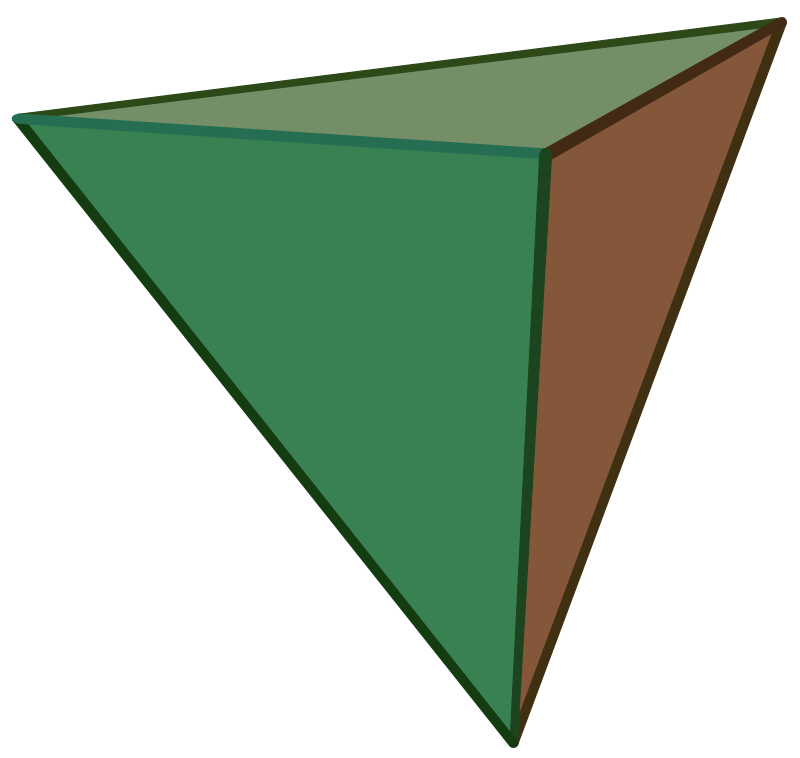
\includegraphics[width=0.45\linewidth]{Tetrahedron}
		\vspace*{-10pt}
	\end{figure}
	có $4$ đỉnh, $6$ cạnh và $4$ mặt. Công thức Euler cho tứ diện là hệ thức sau đây:
	\begin{align*}
		\boxed{4-6+4=2.}
	\end{align*}
	$2.$ Hình lập phương
	\begin{figure}[H]
		\centering
		\vspace*{-5pt}
		\captionsetup{labelformat= empty, justification=centering}
		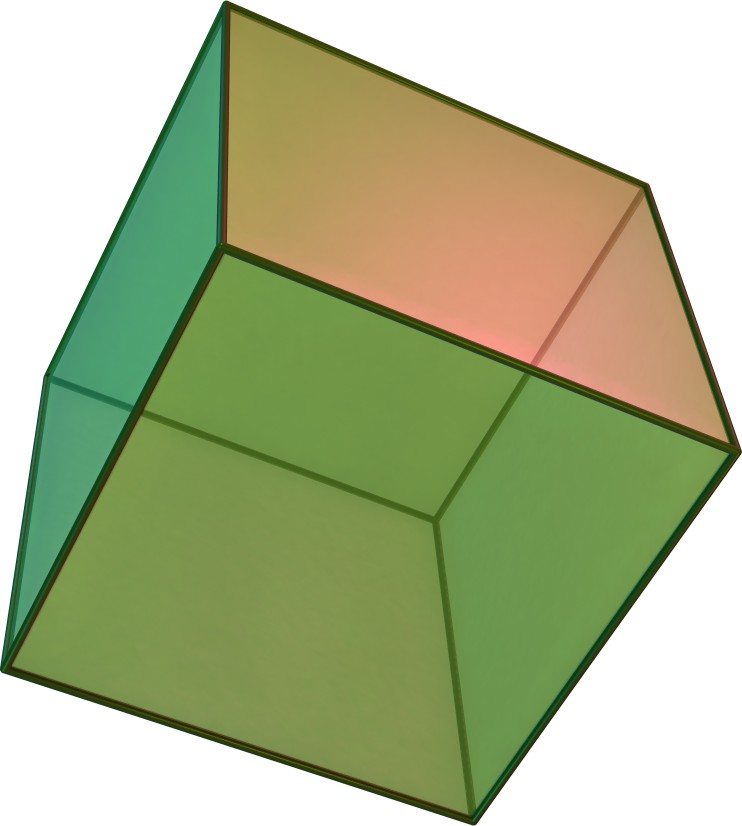
\includegraphics[width=0.45\linewidth]{Hexahedron}
		\vspace*{-10pt}
	\end{figure}
	có $8$ đỉnh, $12$ cạnh và $6$ mặt. Công thức Euler cho tứ diện nói rằng
	\begin{align*}
		\boxed{8-12+6=2.}
	\end{align*}
	$3.$ Kim  tự tháp
	\begin{figure}[H]
		\centering
		\vspace*{-5pt}
		\captionsetup{labelformat= empty, justification=centering}
		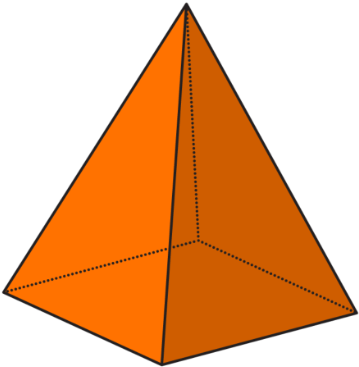
\includegraphics[width=0.45\linewidth]{Pyramid}
		\vspace*{-10pt}
	\end{figure}
	có $5$ đỉnh, $8$ cạnh và $5$ mặt. Trong trường hợp này, công thức Euler khẳng định rằng
	\begin{align*}
		\boxed{5-8+5=2.}
	\end{align*}
	$4.$ Tuy nhiên, đối với hình ba chiều sau, giống như một chiếc phao, còn gọi là ``xuyến lục giác",
	\begin{figure}[H]
		\centering
		\vspace*{-5pt}
		\captionsetup{labelformat= empty, justification=centering}
		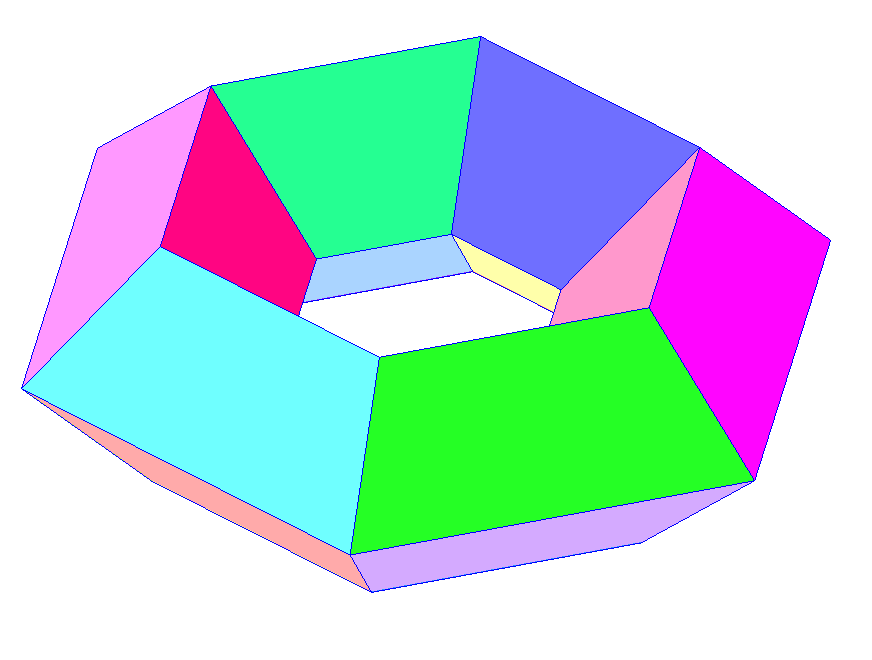
\includegraphics[width=0.5\linewidth]{Hexagonal_torus}
		\vspace*{-10pt}
	\end{figure}
	là một hình khối có $6\times 4=24$ đỉnh, $24+ 24=48$ cạnh và $6\times 4=24$ mặt, trong trường hợp này, công thức Euler không còn đúng nữa, bởi vì
	\begin{align*}
		\boxed{ 24 - 48 + 24 = 0\neq  2}.
	\end{align*}
	Điều này đến từ việc hình khối trên đây không phải là một hình lồi!}
	\vskip 0.1cm
	$\pmb{2.}$ \textbf{\color{hoccungpi}Chứng minh công thức Euler}
	\vskip 0.1cm
	Trong khi công thức Euler ban đầu được phát biểu cho các khối đa diện (lồi),  ngày nay nó thường được phát biểu trong bối cảnh tổng quát hơn với các đồ thị phẳng.
	\vskip 0.1cm
	Nhắc lại rằng một đồ thị là $G=(V, E)$ là một cặp được tạo thành từ một tập đỉnh $V$ và một tập cạnh $E$, trong đó mỗi cạnh được xác định bởi $2$ đầu mút của nó (nghĩa là mỗi cạnh có dạng $e=\{A,B\}$, trong đó  $A, B$ là hai đỉnh nào đó của đồ thị). Chúng ta thường mô tả đồ thị bằng hình vẽ: các đỉnh bởi các điểm và mỗi cạnh bởi một đường cong liên tục nối hai đỉnh với nhau. 
	\vskip 0.1cm
	\textbf{\color{hoccungpi}Ví dụ} $\pmb{2.}$
	\textit{Ta có các ví dụ sau đây về đồ thị $K_5$ (hình bên trái) và $K_{3,3}$ (hình bên phải):}
	\begin{figure}[H]
		\centering
		\vspace*{-5pt}
		\captionsetup{labelformat= empty, justification=centering}
		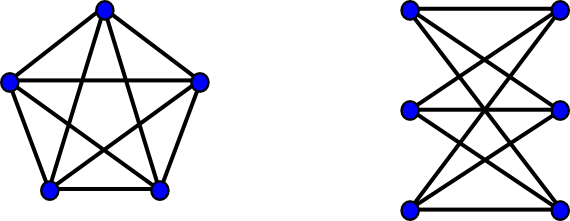
\includegraphics[width=1\linewidth]{k5_n_k33}
		\vspace*{-15pt}
	\end{figure}
	Một \emph{đồ thị phẳng} là một đồ thị mà ta {\emph có thể} vẽ trong mặt phẳng sao cho các cạnh của nó chỉ gặp nhau tại các đỉnh của đồ thị. Lưu ý rằng một đồ thị có thể có nhiều cách vẽ khác nhau (còn gọi là các biểu diễn) và một đồ thị phẳng có thể có các biểu diễn ``không phẳng" -- một biểu diễn hình học mà trong đó các cạnh có thể cắt nhau.
	\vskip 0.1cm
	\textbf{\color{hoccungpi}Ví dụ} $\pmb{3.}$ \textit{Ba hình vẽ sau đây đều là các biểu diễn khác nhau của đồ thị $K_4$: đồ thị có $4$ đỉnh, trong đó hai đỉnh bất kỳ được nối với nhau bằng một cạnh.
	\begin{figure}[H]
		\centering
		\vspace*{-5pt}
		\captionsetup{labelformat= empty, justification=centering}
		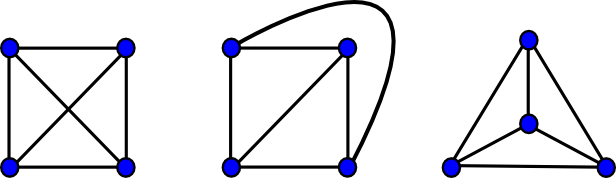
\includegraphics[width=1\linewidth]{K4}
		\vspace*{-15pt}
	\end{figure}
	Tuy nhiên, hình bên trái là một biểu diễn không phẳng và hai hình còn lại là các biểu diễn phẳng. 
	\vskip 0.1cm
	Do đó ta có thể kết luận rằng $K_4$ là một đồ thị phẳng.}
	\vskip 0.1cm
	Nhận xét rằng, một khối đa diện lồi là một đồ thị phẳng. Cụ thể hơn, với một đa diện lồi bất kỳ, đồ thị với các đỉnh là các đỉnh của khối đa diện và các cạnh được cho bởi các cạnh của khối đa diện là một đồ thị phẳng.
	\vskip 0.1cm
	Để chỉ ra điều đó, ta cần chỉ ra đồ thị xây dựng như trên có một biểu diễn phẳng. Có một cách trực quan để thấy điều đó như sau: cắt một trong các mặt của hình đa diện dọc theo các cạnh trên biên của mặt đó và hãy hình dung rằng các mặt còn lại được tạo thành từ cao su (sao cho chúng có thể co giãn được). Sau đó kéo căng hình đa diện có một mặt đã bị  bỏ đi để khiến cho nó trở thành một hình phẳng. Bằng cách đó, ta thu được một biểu diễn phẳng của đồ thị liên kết với khối đa diện. 
	\vskip 0.1cm
	Cho một đồ thị phẳng $G$ và cho một biểu diễn phẳng của $G$. Thế thì các cạnh của $G$ phân chia mặt phẳng thành các miền. 
	\vskip 0.1cm
	Một cách chính xác hơn, một mặt của đồ thị phẳng là một miền cực đại (theo quan hệ bao hàm) không chứa bất kỳ đỉnh cũng như một phần nào của các cạnh của đồ thị. Ta có thể hình dung về các mặt của một đồ thị phẳng một cách trực quan như sau: xét một biểu diễn phẳng của một đồ thị phẳng trên một mảnh giấy, sau đó, lấy kéo cắt dọc theo các cạnh của đồ thị, thế thì các mảnh giấy rời ra chính là các mặt của đồ thị phẳng.
	\vskip 0.1cm
	Ta có thể nhận thấy rằng, với một biểu diễn phẳng của một đồ thị phẳng, có duy nhất một mặt là không bị chặn (các cạnh bao quanh nó tạo thành một đường khép kín, hay một chu trình), còn các mặt còn lại, nếu có, là các mặt bị chặn (các cạnh bao quanh nó tạo thành một chu trình).
	\vskip 0.1cm
	\textbf{\color{hoccungpi}Ví dụ} $\pmb{4.}$
	\textit{$1.$ Đồ thị con bướm
	\begin{figure}[H]
		\centering
		\vspace*{-5pt}
		\captionsetup{labelformat= empty, justification=centering}
		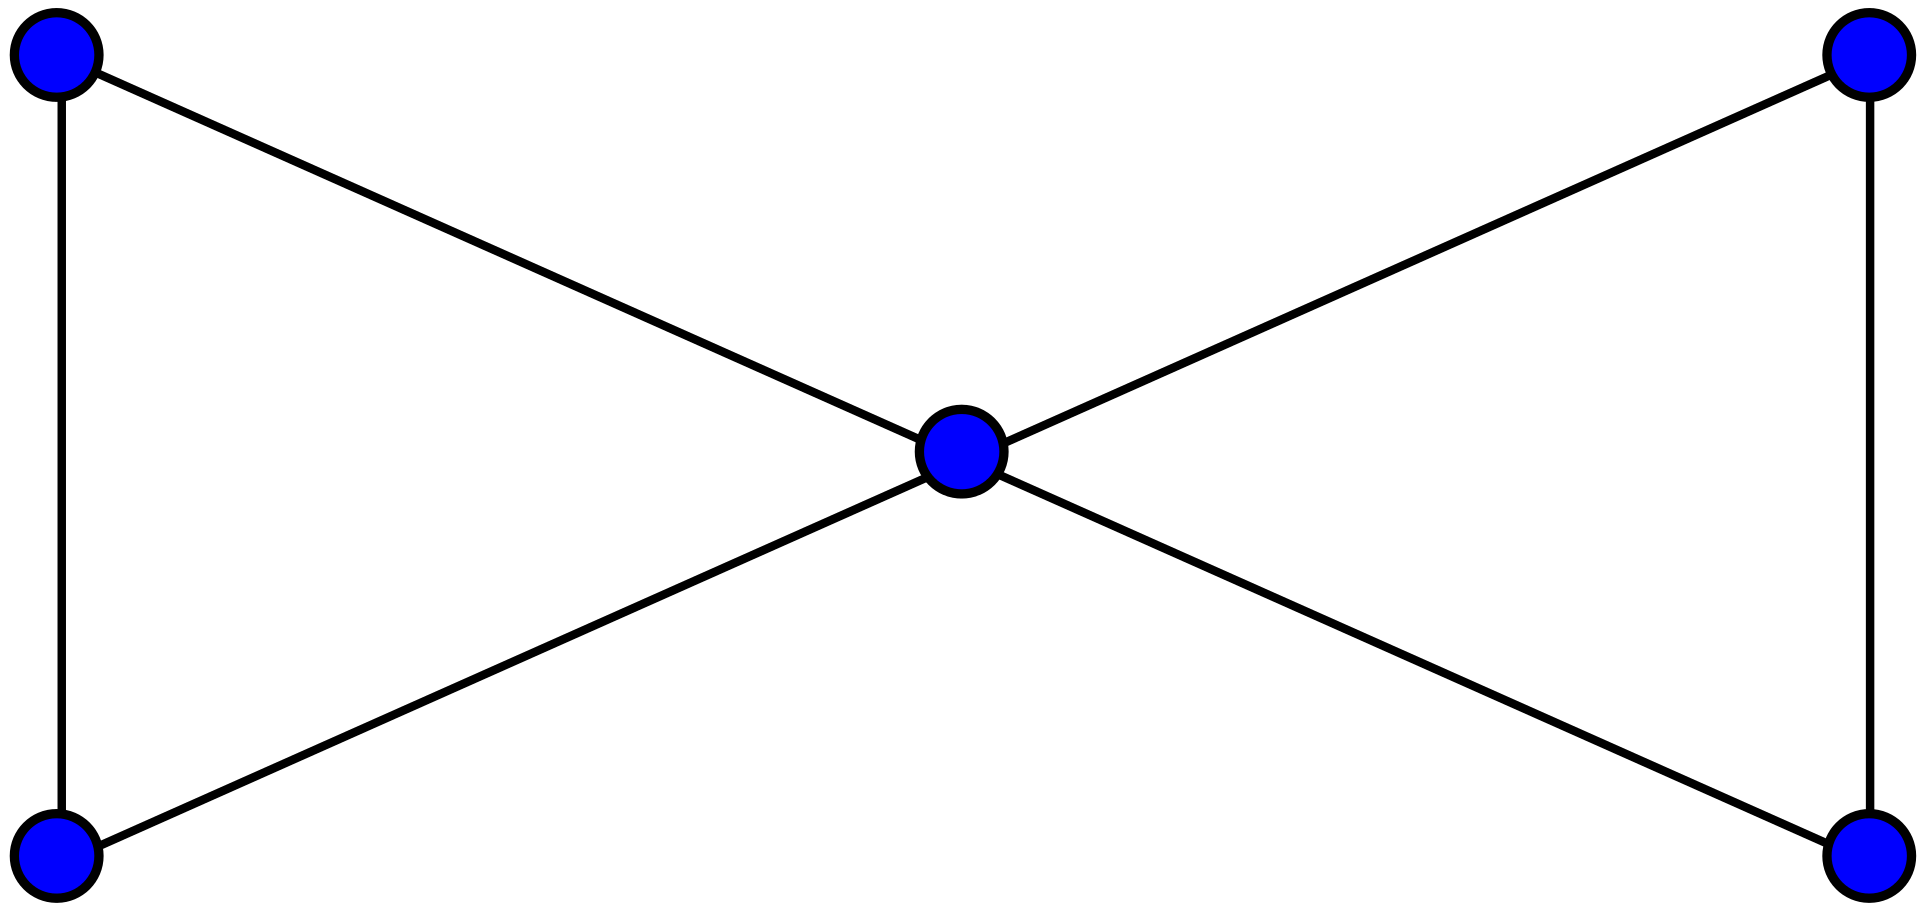
\includegraphics[width=0.6\linewidth]{Butterfly}
		\vspace*{-10pt}
	\end{figure}
	là một đồ thị phẳng có $5$ đỉnh, $6$ cạnh và $3$ mặt (gồm $2$ mặt bị chặn là các tam giác và $1$ mặt không bị chặn).
	\vskip 0.1cm
	$2.$  Đồ thị $K_4$
	\begin{figure}[H]
		\centering
		\vspace*{-5pt}
		\captionsetup{labelformat= empty, justification=centering}
		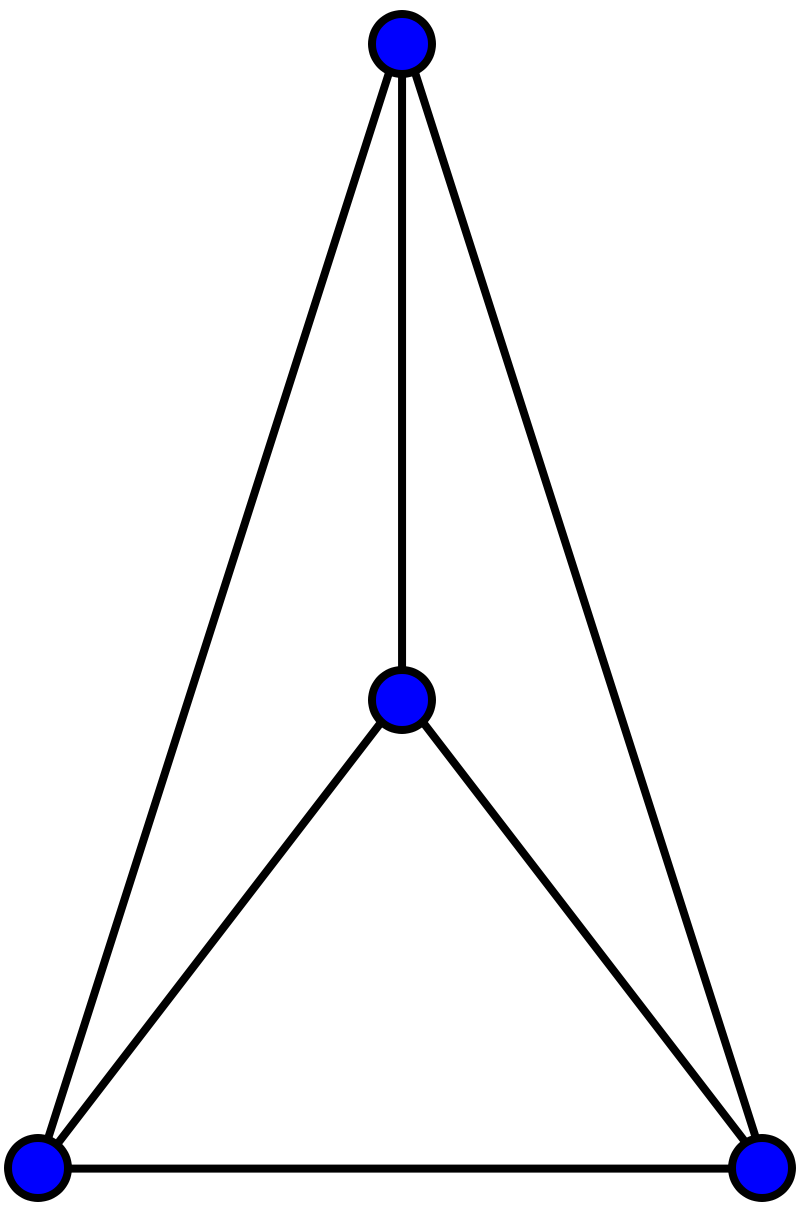
\includegraphics[width=0.4\linewidth]{K4b}
		\vspace*{-5pt}
	\end{figure}
	là một đồ thị phẳng có $4$ đỉnh, $6$ cạnh và $4$ mặt (gồm $3$ mặt bị chặn là các tam giác và $1$ mặt không bị chặn).}
	\vskip 0.1cm
	Bây giờ, ta đã sẵn sàng để phát biểu công thức Euler cho đồ thị phẳng.
	\vskip 0.1cm
	\textbf{\color{hoccungpi}Định lý} $\pmb{2.}$ (Công thức Euler cho đồ thị phẳng)\textbf{\color{hoccungpi}.} \textit{Cho $G$ là một đồ thị phẳng liên thông  với $v$ đỉnh, $e$ cạnh. Giả sử $f$ là số mặt của một biểu diễn phẳng (bất kỳ) của $G$. Thế thì}
	\begin{align*}
		v-e + f =2.
	\end{align*}
	Nhắc lại rằng một đồ thị được gọi là liên thông nếu ta có thể di chuyển theo các cạnh để đi từ một đỉnh bất kỳ tới một đỉnh bất kỳ khác.
	\vskip 0.1cm
	\textit{Chứng minh.} Hãy coi mặt vô hạn (miền của mặt phẳng không bị chặn) của biểu diễn phẳng của $G$ là đại dương, các cạnh của biểu diễn phẳng là những con đê làm bằng đất và các mặt bị chặn là những cánh đồng khô. Dưới đây là một ví dụ điển hình của đồ thị phẳng liên thông.
	\begin{figure}[H]
		\centering
		\vspace*{-5pt}
		\captionsetup{labelformat= empty, justification=centering}
		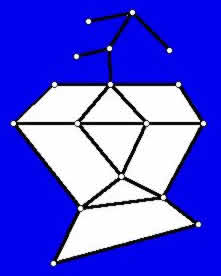
\includegraphics[width=0.5\linewidth]{proof_Euler_1}
		\vspace*{-10pt}
	\end{figure}
	Trong hình vẽ bên dưới, một cạnh nằm trên biên của một mặt bị chặn được tô đỏ và cạnh này tiếp giáp với đại dương. Khi con đê đại diện bởi cạnh màu đỏ này bị ``phá vỡ", cánh đồng ở phía bên kia của con đê được thông ra biển và trở nên ngập nước, được minh họa bằng màu xanh ngọc (cho dù đúng ra nó phải có màu xanh lam của đại dương).
	\begin{figure}[H]
		\centering
		\vspace*{5pt}
		\captionsetup{labelformat= empty, justification=centering}
		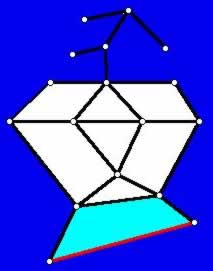
\includegraphics[width=0.5\linewidth]{proof_Euler_2}
		\vspace*{-10pt}
	\end{figure}
	Nếu đồ thị liên thông có các mặt bị chặn (biên của các mặt như vậy là các đường khép kín: các chu trình),  ta có thể loại bỏ một cạnh khỏi mỗi mặt này mà vẫn bảo toàn tính chất liên thông của đồ thị (và tất nhiên tính phẳng cũng vậy). 
	\vskip 0.1cm
	Ta dễ dàng nhận nhận thấy có một song ánh giữa các cạnh bị bỏ đi để nhận được một đồ thị liên thông, không có chu trình và các mặt bị chặn của đồ thị. Trong hình vẽ sau, các cạnh bị bỏ đi được tô bằng bằng màu đỏ và các cánh đồng ngập nước được hiển thị bằng màu xanh ngọc.
	\begin{figure}[H]
		\centering
		\vspace*{-5pt}
		\captionsetup{labelformat= empty, justification=centering}
		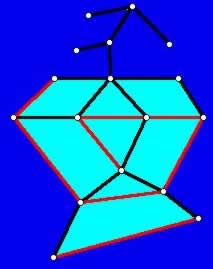
\includegraphics[width=0.5\linewidth]{proof_Euler_3}
		\vspace*{-10pt}
	\end{figure}
	Đồ thị nhận được sau cùng, có cùng tập đỉnh với đồ thị ban đầu và các cạnh còn lại màu đen, được gọi là một \emph{cây bao trùm} của đồ thị ban đầu.  (Do đó, một cây bao trùm của một đồ thị liên thông có cùng số đỉnh với đồ thị ban đầu, nhưng ít cạnh hơn, trừ khi bản thân đồ thị ban đầu là một cây.) Theo định nghĩa, một cây là một đồ thị liên thông và không có chu trình. 
	\vskip 0.1cm
	Chẳng hạn, ba đồ thị đầu tiên là một cây, còn đồ thị ngoài cùng bên phải không phải là cây.
	\begin{figure}[H]
		\centering
		\vspace*{5pt}
		\captionsetup{labelformat= empty, justification=centering}
		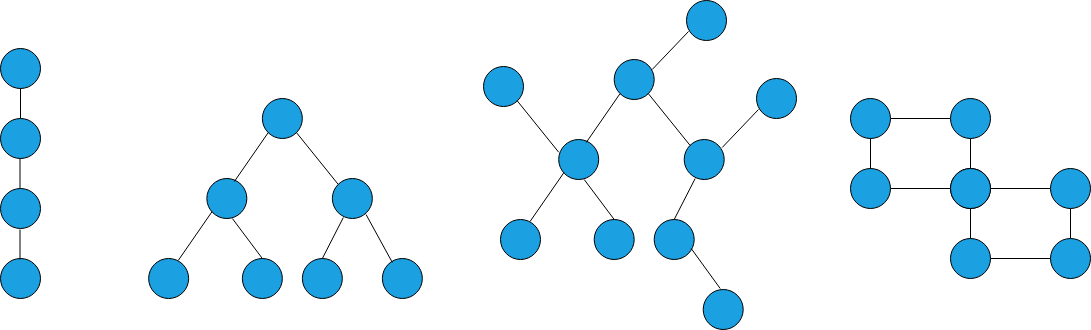
\includegraphics[width=1\linewidth]{trees}
		\vspace*{-10pt}
	\end{figure}
	Ta có kết quả quen thuộc sau đây: với một cây bất kỳ, số cạnh và số đỉnh của nó được ràng buộc với nhau bởi hệ thức: 
	\begin{align*}
		\boxed{v = e + 1.}
	\end{align*}
	Chứng minh của kết quả này có thể được tìm thấy trong nhiều tài liệu về lý thuyết đồ thị. Tuy nhiên, tác giả của bài viết khuyên các bạn đọc quan tâm tự chứng minh kết quả trên.
	\vskip 0.1cm
	Bây giờ, chúng ta hãy đếm các cạnh của đồ thị ban đầu bằng cách cộng số cạnh bị loại bỏ (để thu được một cây) với các cạnh còn lại (của cây nhận được).  Các cạnh bỏ đi chính là các cạnh màu đỏ và các cạnh còn lại chính là các cạnh màu đen. Vì vậy, số cạnh của đồ thị ban đầu là
	\begin{align*}
		e = e_{\textrm{đỏ}} + e_{\textrm{đen}}.
	\end{align*}
	Bây giờ, một mặt, chúng ta biết rằng $e_{\textrm{đỏ}}=f-1$: điều này là bởi vì chúng ta cần bỏ đi một cạnh màu đỏ để làm ngập mỗi vùng khô (chính là các mặt bị chặn) và đồ thị còn lại có (duy nhất) một mặt không bị chặn ngoài các mặt bị chặn đã xét đến. Mặt khác, ta có $e_{\textrm{đen}}=v-1$ bởi vì các cạnh màu đen tạo thành một cây bao trùm của đồ thị ban đầu. Suy ra
	\begin{align*}
		e = f-1 + v-1,
	\end{align*}
	có nghĩa là $v-e+f=2$.
	\vskip 0.1cm
	$\pmb{3.}$ \textbf{\color{hoccungpi}Ứng dụng của công thức Euler trong phân loại các khối đa diện đều}
	\vskip 0.1cm
	Một khối đa diện (lồi) được gọi là đều nếu các mặt của nó là các đa giác đều bằng nhau và số cạnh đi ra từ mỗi đỉnh của đa diện có là bằng nhau. Việc phân loại các đa diện đều được biết đến từ thời Platon. Ta có kết quả quen thuộc sau đây.
	\vskip 0.1cm
	\textbf{\color{hoccungpi}Định lý} $\pmb{3.}$ \textit{Có tất cả $5$ loại khối đa diện đều. Đó là: hình tứ diện đều, hình lập phương, hình bát diện đều, hình mười hai mặt đều, hình hai mươi mặt đều.}
	\begin{figure}[H]
		\centering
		\vspace*{-5pt}
		\captionsetup{labelformat= empty, justification=centering}
		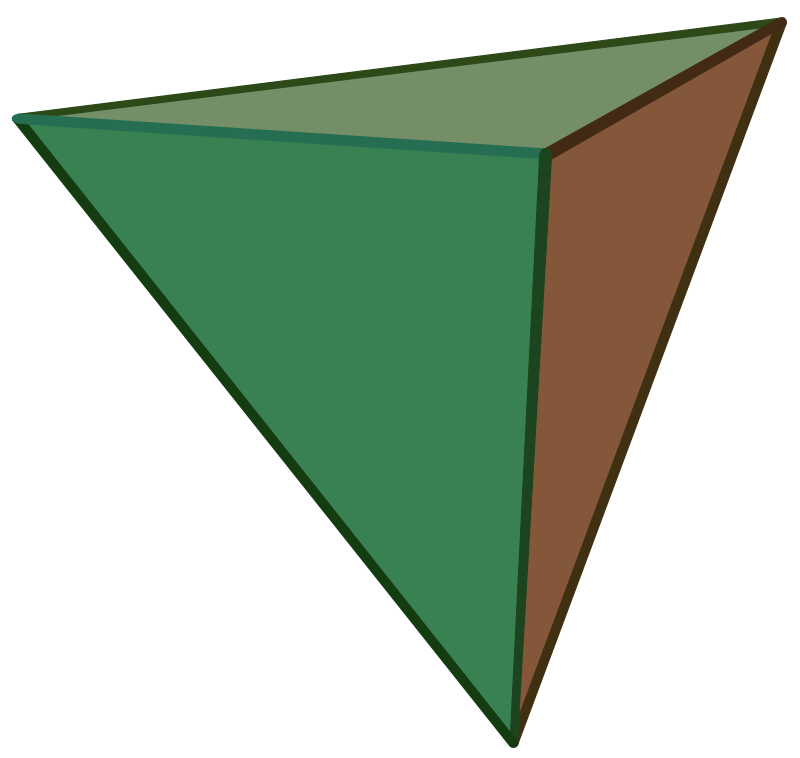
\includegraphics[scale=0.07]{Tetrahedron.png} 
		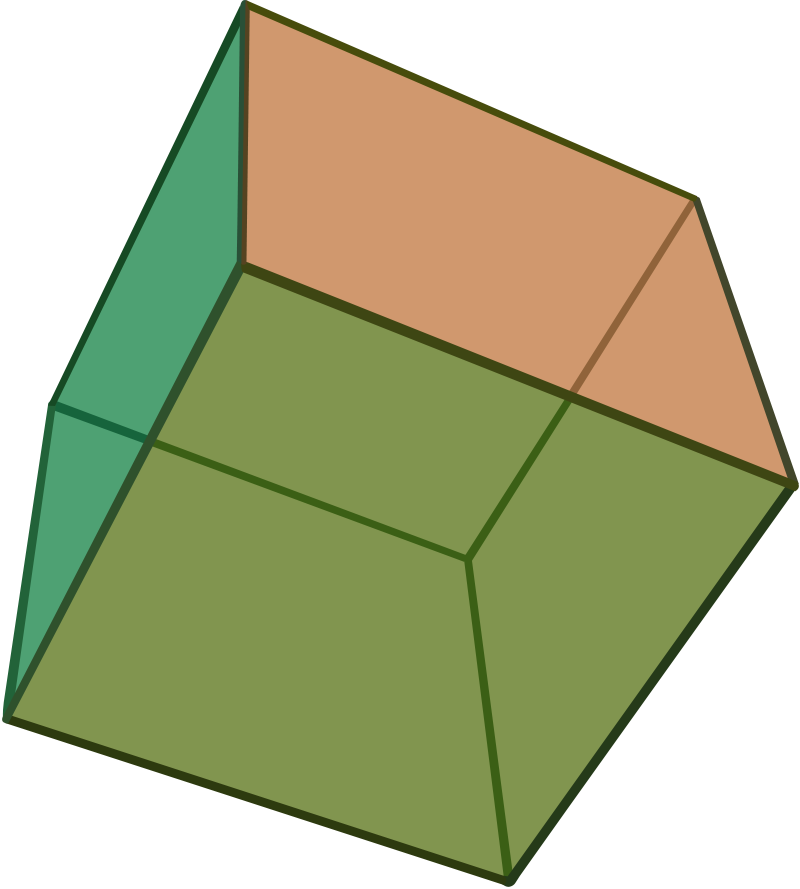
\includegraphics[scale=0.07]{Hexahedron.png}
		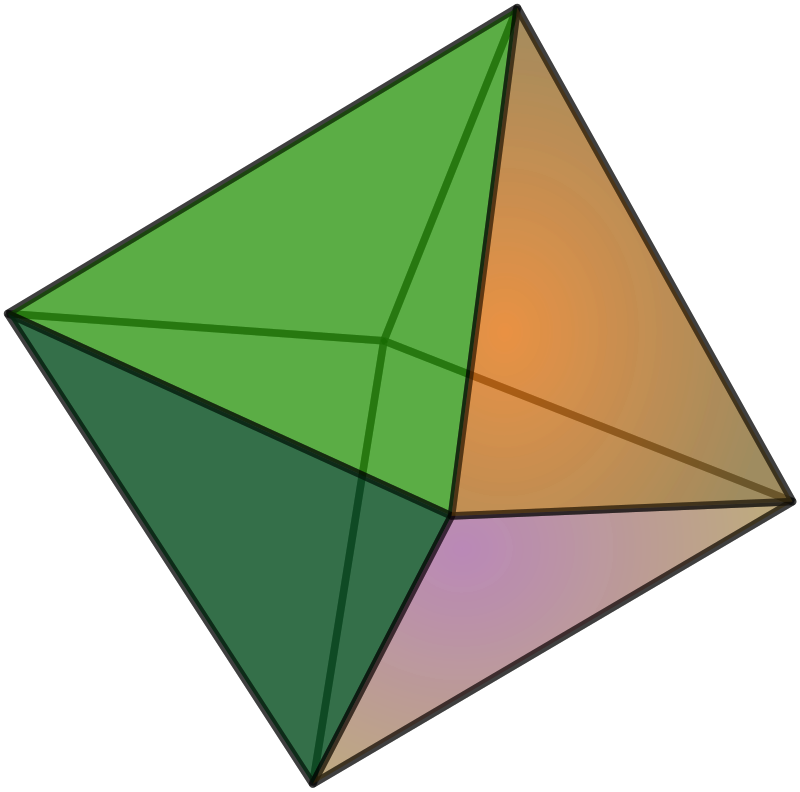
\includegraphics[scale=0.07]{Octahedron.png}
		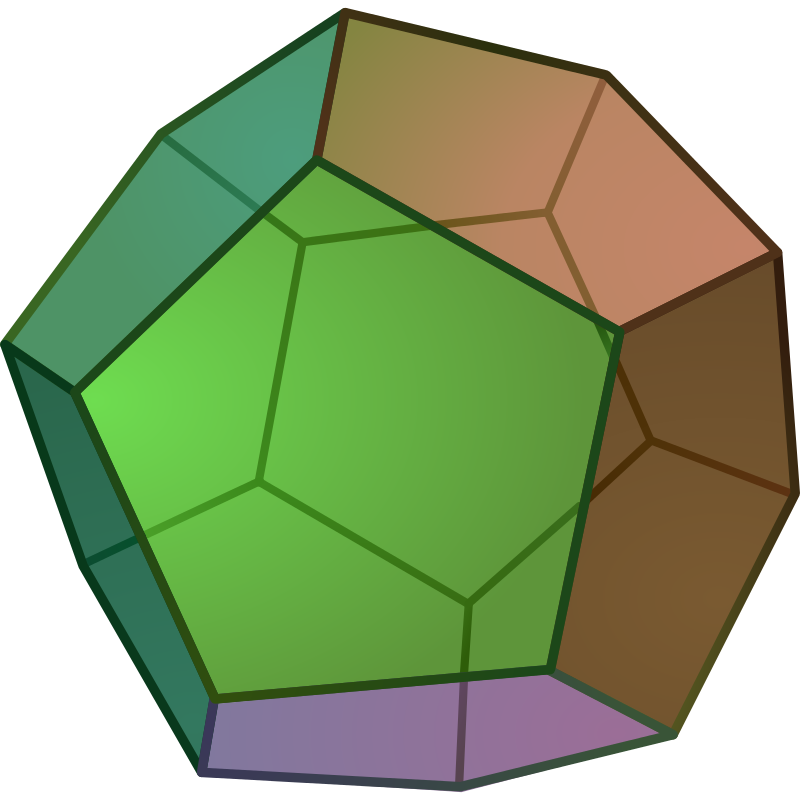
\includegraphics[scale=0.07]{Dodecahedron.png}
		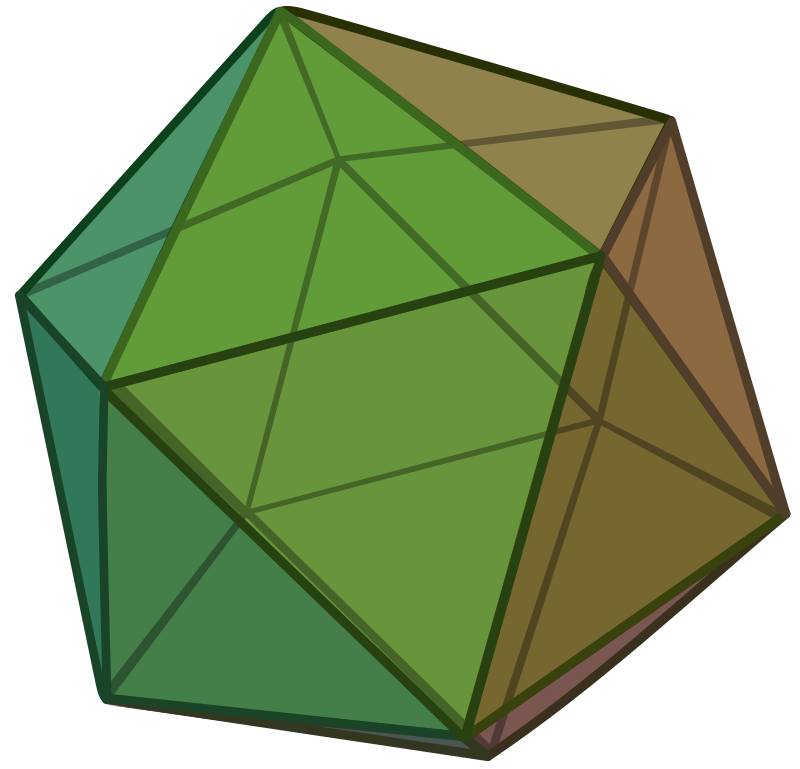
\includegraphics[scale=0.07]{Icosahedron.png}
		\vspace*{-10pt}
	\end{figure}
	\textit{Chứng minh.} Xét một khối đa diện đều $P$. Giả sử $P$ có $v$ đỉnh và mỗi đỉnh có bậc $k$ (nghĩa là mỗi đỉnh có $k$ cạnh đi ra từ đó) và mỗi mặt là một đa giác đều có $m$ cạnh. Gọi $e, f$ tương ứng là số cạnh và số mặt của $P$. 
	\vskip 0.1cm
	$\bullet$ Một mặt, ta có $kv= 2e$: mỗi đỉnh có $k$ cạnh đi ra, do đó có tổng cộng $kv$ cạnh, nhưng mỗi cạnh được đếm $2$ lần.
	\vskip 0.1cm
	$\bullet$ Mặt khác, $m f=2e$: mỗi mặt có $m$ cạnh, do đó có $mf $ cạnh, nhưng mỗi cạnh cũng được đếm $2$ lần do mỗi cạnh nằm trên đúng $2$ mặt.
	\vskip 0.1cm
	Suy ra $v = \frac{2e}{k}, f = \frac{2e}{m}$. Thay vào công thức Euler cho đa diện: $v-e+f=2$, ta có 
	\begin{align*}
		e\left(\frac{2}{k}-1 + \frac{2}{m}\right)=2.
	\end{align*}	
	Nói riêng, $\frac{2}{k}-1 + \frac{2}{m} >0$, hay $(k-2)(m-2) < 4$.
	\vskip 0.1cm	
	Chú ý rằng $k \geq 3, m \geq 3$ do mỗi đỉnh phải có ít nhất $3$ cạnh đi ra từ đó và mỗi mặt có ít nhất $3$ cạnh. Kết hợp với bất đẳng thức $(k-2)(m-2) < 4$ ta suy ra $3 \leq k, m \leq 5$. Thử lại ta thấy các bộ thỏa mãn các bất đẳng thức trên là 
	\begin{align*}
		\boxed{(k, m)\!\in\! \{\!(3,3), (3, 4), (3, 5), (4, 3), (5, 3)\!\}\!.}
	\end{align*}
	Đảo lại, ứng với các giá trị này ta có các đa diện đều: khối tứ diện đều, khối lập phương, khối bát diện đều, khối mười hai mặt đều và khối hai mươi mặt đều.
	\vskip 0.1cm
	$\pmb{4.}$ \textbf{\color{hoccungpi}Một số ví dụ ứng dụng khác của công thức Euler}
	\vskip 0.1cm
	Ta có bài toán đố nổi tiếng sau đây.
	\vskip 0.1cm
	\textbf{\color{hoccungpi}Ví dụ} $\pmb{5.}$ \textit{Trong một thị trấn có $3$ ngôi nhà $A, B, C$ và ba nhà máy điện, nước và khí đốt. Mỗi ngôi nhà cần phải được nối với mỗi nhà máy trên bởi một đường ống. Hỏi có thể xây dựng được các đường ống sao cho hai đường ống đôi một không giao nhau hay không?}
	\begin{figure}[H]
		\centering
		\vspace*{-5pt}
		\captionsetup{labelformat= empty, justification=centering}
		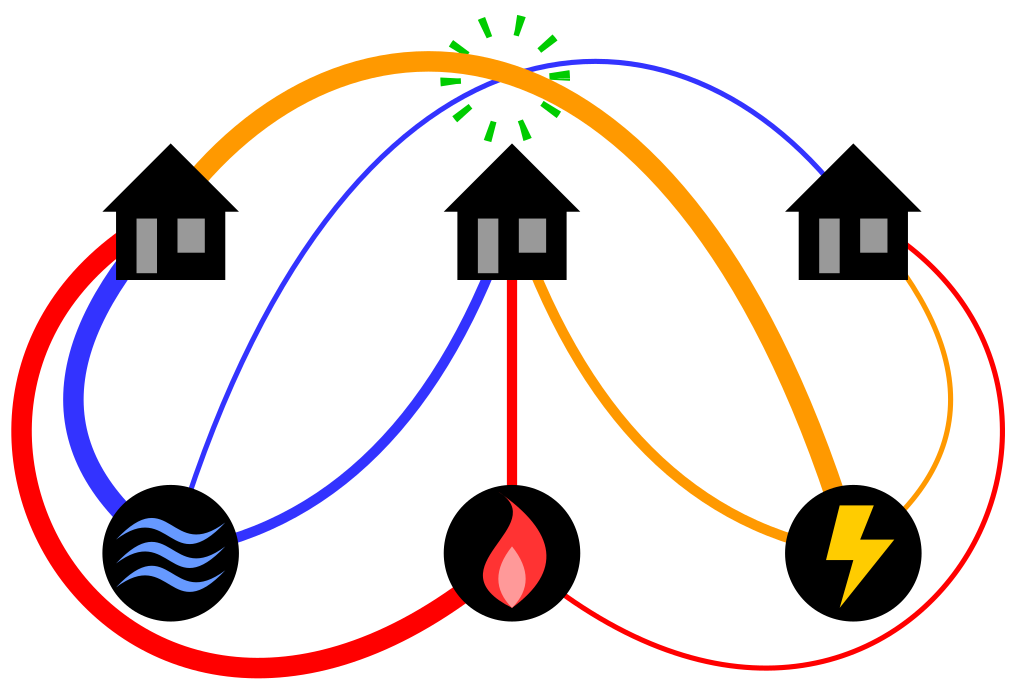
\includegraphics[width=1\linewidth]{3_utilities}
		\vspace*{-10pt}
	\end{figure}
	\textit{Lời giải.} Biểu diễn các ngôi nhà và các nhà máy bằng các điểm của mặt phẳng và các đường ống bằng các đường liên tục. Ta thu được một đồ thị gồm $6$ đỉnh ($3$ ngôi nhà và $3$ nhà máy) và $9$ cạnh (nối mỗi ngôi nhà với mỗi nhà máy).  Bài toán yêu cầu chứng minh đồ thị nhận được, được gọi là đồ thị $K_{3, 3}$, không phải là đồ thị phẳng.
	\begin{figure}[H]
		\centering
		\vspace*{-5pt}
		\captionsetup{labelformat= empty, justification=centering}
		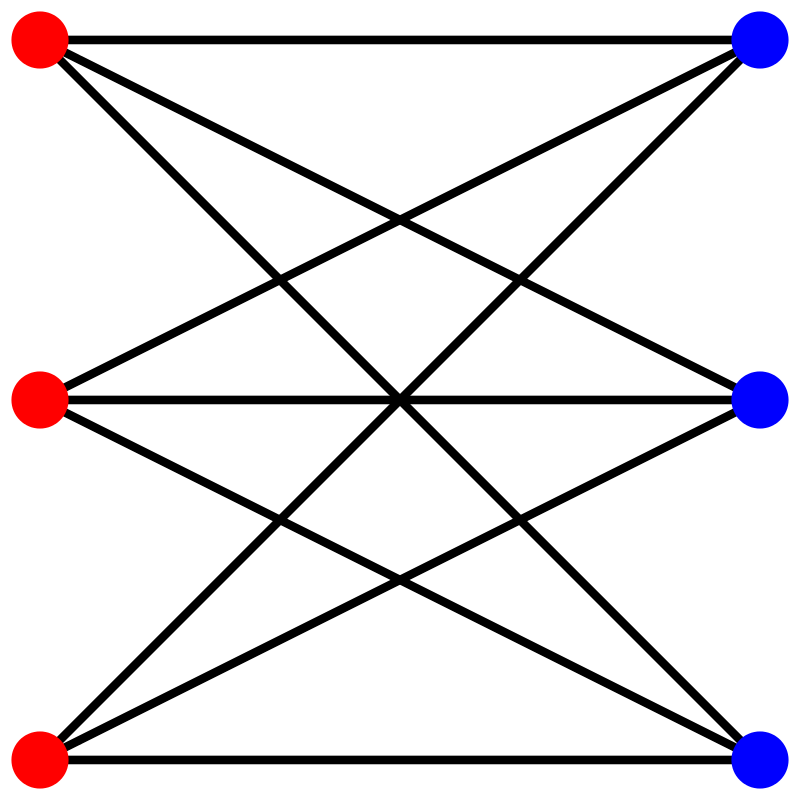
\includegraphics[scale=0.15]{K3_3}
		\vspace*{-10pt}
	\end{figure}
	Giả sử ngược lại, đồ thị $K_{3,3}$ là một đồ thị phẳng có $f$ mặt. 
	\vskip 0.1cm
	$\bullet$ Theo công thức Euler, ta có
	\begin{align*}
		6 - 9 + f = 2.
	\end{align*}
	Suy ra $f=5$.
	\vskip 0.1cm
	$\bullet$  Mặt khác, dễ thấy không một mặt nào, bị chặn hay không bị chặn, của $K_{3, 3}$ là tam giác (do các cạnh chỉ nối các nhà máy với các ngôi nhà, chứ không nối $2$ nhà máy với nhau cũng như $2$ ngôi nhà với nhau). Từ đó suy ra mỗi mặt của $K_{3,3}$ có ít nhất $4$ cạnh. Mà mỗi cạnh thuộc đúng hai mặt. Chứng tỏ $2$ lần số cạnh $ \geq $ $4$ lần số mặt. Suy ra $f \leq \frac{9}{2}$, mâu thuẫn với việc $f=5$.
	\vskip 0.1cm
	Bài toán về trò chơi sau đây được lấy từ kỳ thi Putnam, một kỳ thi Toán dành cho sinh viên các trường đại học của Mỹ. 
	\vskip 0.1cm
	\textbf{\color{hoccungpi}Ví dụ} $\pmb{6.}$
	\textit{Cho một đa diện với ít nhất $5$ mặt và sao cho mỗi đỉnh có đúng $3$ cạnh xuất phát từ đó. Hai bạn $A$ và $B$ chơi trò chơi sau đây trên đa diện đó: mỗi người lần lượt, bạn $A$ bắt đầu, viết tên mình lên một mặt chưa từng được viết lên. Người chiến thắng là người đầu tiên viết tên mình lên $3$ mặt cùng chung $1$ đỉnh. Hỏi ai là người có chiến lược thắng cuộc?}
	\vskip 0.1cm
	\textit{Lời giải}
	Trả lời: bạn $A$ có chiến lược thắng!
	\vskip 0.1cm	
	Nếu tồn tại một mặt $F_0$ với ít nhất $4$ cạnh thì $A$ viết tên lên mặt đó. Giả sử $F_0$ có các cạnh $e_1, \ldots,e_k (k\geq 4)$. Nếu $B$ viết lên một cạnh kề với $F_0$, có nghĩa là một trong các mặt $F_i$, mặt chung cạnh $e_i$ với $F_0$. Không mất tính tổng quát, gọi đó là mặt $F_1$. Thế thì lượt tiếp theo, $A$ viết lên mặt $F_3$. Khi đó, ở lượt tiếp theo, $B$ không thể ngăn $A$ viết lên một trong $2$ mặt $F_2, F_4$. (Tất nhiên, $A$ giữ chiến lược này cả khi $B$ không chọn một mặt kề với $F_0$.)
	\vskip 0.1cm
	Giả sử đa diện không có mặt có $\ge 4$ cạnh. Thế thì mỗi mặt là một tam giác. Nhưng một đa diện có mỗi mặt là một tam giác và mỗi đỉnh có bậc $3$ phải là một tứ diện.Thật vậy điều này được suy ra từ các đẳng thức: $v-e+f=2$ (công thức Euler), $2e=3f$ (vì mỗi mặt là một tam giác) và $2e=3v$ (vì mỗi đỉnh có bậc $3$). Nhưng điều này mâu thuẫn với giả thiết rằng đa diện có $\geq 5 $ mặt. 
	\vskip 0.1cm
	Công thức Euler có vai trò quan trọng trong một số bài toán thi học sinh giỏi ở bậc phổ thông. Chẳng hạn, bài toán sau đây xuất hiện trong đề thi Olympic Toán học Trung Quốc lần thứ $36$, năm $2020-2021$.
	\vskip 0.1cm
	\textbf{\color{hoccungpi}Ví dụ} $\pmb{7.}$ \textit{Cho $P$ là một khối đa diện thỏa mãn: 
	\vskip 0.1cm
	$\bullet$ Mỗi đỉnh của $P$ thuộc ba mặt khác nhau;
	\vskip 0.1cm
	$\bullet$ Với mọi số nguyên $ k \geq 3$, số mặt của $P$ có $k$ cạnh là một số chẵn.
	\vskip 0.1cm
	$\bullet$ Một con kiến bò dọc theo các cạnh của $P$, bắt đầu từ trung điểm của một cạnh, bò theo một hành trình khép kín $L$, đi qua mỗi điểm trên $L$ đúng một lần, và cuối cùng quay trở lại điểm xuất phát. Hành trình $L$ chia bề mặt của đa diện $P$ thành $2$ phần, sao cho với mọi $k \leq 3$, số đa giác $k$ cạnh trong hai phần đó là bằng nhau. Chứng minh số lần rẽ trái và rẽ phải của con kiến là bằng nhau.}
	\vskip 0.1cm
	Bạn đọc hãy tự thử sức mình với bài toán trên. Lời giải của bài toán có thể được tìm thấy trong Tạp chí Pi, số $3$ năm $2022$.
	\vskip 0.1cm
	\textbf{\color{hoccungpi}Tài liệu}
	\vskip 0.1cm
	[$1$] Nguyễn Hữu Việt Hưng. \emph{Rộng hẹp nhỏ to đều vậy cả (hay Tôpô học là gì?)} Tạp chí Pi, tập $2$, số $7$ năm $2018$.
	\vskip 0.1cm
	[$2$] Joseph Malkevitch. \emph{Euler's polyhedral formula}. Notices of the American Mathematical Society, số $12$ năm $2004$.
\end{multicols}